\documentclass{article}

\title{EW309 Final Report, Team Anglerfish One}
\author{T Hendricks and P Malatesta}
\date{\today}

\usepackage{siunitx}
\usepackage{graphicx}
\bibliographystyle{IEEEtran}
\usepackage{amsmath,amsfonts,amssymb}
\usepackage{listings}
\lstset{%
    basicstyle=\small\ttfamily,
    columns=fullflexible,
    showstringspaces=false}
\usepackage{hyperref}
\usepackage[dvipsnames,svgnames]{xcolor}
\hypersetup{%
    colorlinks=true,
    linkcolor=violet,
    urlcolor=blue,
    citecolor=blue}
\usepackage{booktabs}
\usepackage[plain]{fancyref}
\newcommand{\Matlab}{Matlab}

\begin{document}
\maketitle

\begin{abstract}
The system must autonomously scan for, identify, and track discrete targets. Once a target is identified, the turret must center itself on target and, if the turret has a reasonable chance to hit the target, fire. The system must be able to distinguish between valid targets and those that should not be fired upon, and operate accordingly. Though the actual hardware turret was never completed due to global pandemic, a simulated turret was created that could identify and aim at an orange target. The system would calculate the number of shots required to give a certain likelihood of hitting the target, then fire.
% suggestion guys the abstract would normally also say, as a quick summary, what all was achieved in the end. For this reason I often write
% the abstract as the very last thing... 
\end{abstract}

{\scriptsize \textbf{Keywords:} computer vision, ballistics, transfer function}
% these are often used for automatic indexing and retrieval... fill in ones that make sense for you. 

\section{Introduction}
\subsection{Problem statement}
The purpose of EW309 Guided Design is to simulate a capstone project, with extra help to become familiar with the process. The design goal of the class was to create a turret capable of detecting and engaging specific targets with the given constraints. 

% this next one should be the benchmarking, and wants to end with a table or something summarizing/comparing the existing design to your desired design
% moved to abstract
%The system must autonomously scan for, identify, and track discrete targets. Once a target is identified, the turret must center itself on target and, if the turret has a reasonable chance to hit the target, fire. The system must be able to distinguish between valid targets and those that should not be fired upon, and operate accordingly..


\subsection{Existing designs}
% Instructor comment: Maybe comment why all your design comparisons are from Instructables.
% Also add a figure showing the 4 designs you researched and refer to it in the text. 
We turned to instructables to find existing examples of turret designs to compare their features to our constraints. Instructables hosts DIY projects from people around the world, giving good documentation on how different projects operate, and what materials they consist of.
\subsubsection{Instructables Autonomous Sentry Turret}
This turret\footnote{\url{https://www.instructables.com/id/Autonomous-Sentry-Turret/}} design uses a laser range finder and infrared motion sensor to determine targets. The turret sweeps a range of 100 degrees with 10 degree intervals, storing range data. Once data is recorded for the entire sweep and stored data, the turret starts sweeping the same range, and if the range is different from the stored value, the turret fires a third of its clip down the bearing. The turret then waits for the moment sensor to be tripped to begin sweeping again.

The greatest issue this turret has with our problem statement is a lack of discrimination. A difference in rangefinder data will trigger the turret, for example, a door that was either opened or closed mid sweep would be treated as a target. Also, if a person were to walk by the turret during its initial sweep, when the ranges are being determined, the turret would, on its second sweep register a target and begin firing. Furthermore, once the turret starts to fire, the bearing is static, so many shots would be wasted on a moving target. If instead a change in range was coupled with the IR sensor, the system could avoid some false positives.

\subsubsection{Instructables Face Tracking Pan-Tilt Camera}
This\footnote{\url{https://www.instructables.com/id/Face-Tracking-Pan-Tilt-Camera/}} is a gimbal system for a camera meant to track faces (or other objects depending on training). The system must be provided with several photos of whatever image it is meant to detect. The system uses machine learning to determine what constitutes a face (or target of choice), then gives the coordinates of the target relative to the camera’s center. This data is then used to center the servo, using a proportional control.
        
The low point of this solution seems to be the control algorithm. The demonstration videos show slow and imperfect response (with a large steady state error). Furthermore, the system in this project is only built to be able to detect one type of target at a time. It can only positively identify one type of target, and cannot determine between different types of targets. Furthermore, having more than one target in frame could cause the system to oscillate between the two.

\subsubsection{Instructables Portal Turret}
This\footnote{\url{https://www.instructables.com/id/Building-a-moving-and-tracking-Portal-Turret/}} is a 3D printed turret system that can be operated in two modes autonomously or by joystick controlled. When connected to a computer it uses software to detect and track a target designated target. It does this by constantly taking a stream of data and converting it to motor movement. The turret is smart enough to recognize when the target is moving and when the target moves out of the view of the camera.  The software that runs this turret is highly similar to the one that we will use in our own project except it is written in Arduino. 

The biggest weakness of the design however is that it requires the use of a 3D printer to make the pieces with enough precision that the guns, motors, and  electrical work can all fit within the shell. Another issue with this design for our project is it would require us to learn a new language to code the turret.  

\subsubsection{Instructables Robotic Talking Turret}
This turret design\footnote{\url{https://www.instructables.com/id/Robotic-Talking-Turret/}} uses a rangefinder along with the Stampy method to track targets. The rangefinder is constantly sweeping back and forth until it finds a target. Once the target is found the turret starts sweeping and firing. The design of the turret also allows it to know when it is being picked up or tipped over. Both of these actions would stop the rangefinder from moving. 
The largest issues in this design is that it will track and fire at an object whether it be a target or not as long as it is within the set range of the range finder. Meaning that if someone where to walk past or another object be within the set range the turret would track it and fire. Another large issue that this design has is that it fires as soon as an object is within range no matter where the turret is a lined.

% instructor comment: Probably need something here like a table or chart comparing the designs with yours alongside
 % If you prefer you can split your report into smaller files and input them this way... 

\subsection{Target design specifications}
The design was created to detect orange circular targets, and using negative feedback center the turrets firing point on the target, then fire the requisite number of shots to hit the target. The system must be able to accurately and discriminatorily identify, track, and fire upon targets.


\section{System design}
\subsection{Functional block diagram}
\begin{figure}
    \centering
    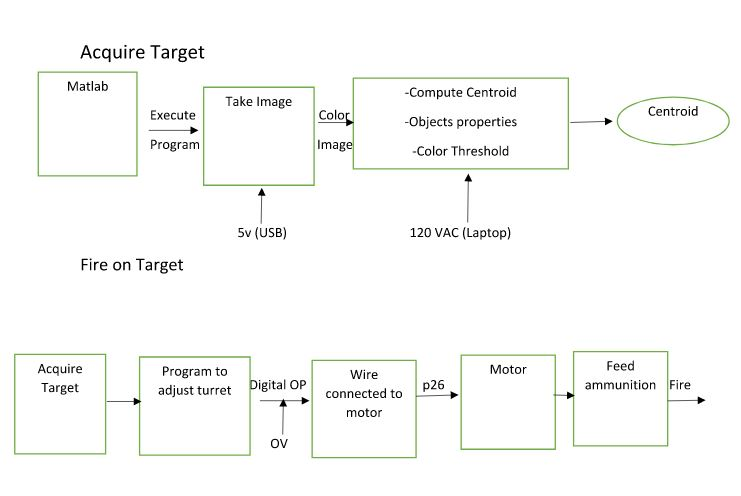
\includegraphics[height=5cm width=4cm]{overall block diagram.JPG}
    \caption{Functional Block Diagram}
    \label{fig:fun diagr}
\end{figure}
The system was designed to find a designated target then a line the turret to said target and fire a bullet. It does this by using computer vision to isolate the target from surrounding and locate it in reference to the center of the turret. Once the target is acquired a voltage is sent to the turret based transfer function that was created to control it's movement.Once the turret reaches a steady state on the target it will determine whether it can hit the target. If it is possible for the turret to hit the target it will then begin to fire a set number of shots at the target. 
 

\subsection{Computer vision}
% This section needs cleaning up
% Probably want a short description of the hardware and a block diagram 

The system uses a pico usb webcam mounted above on a rail above the barrel.
  
Camera mount

% This part explains software processing steps; should go with a block diagram
To get an image into matlab, we initialized a usb webcam, then pulled the color data from a frame taken by the camera. Every loop of the program, we pull a new image, display its color data, and pass that color data on to our thresholding function.

Once an image is acquired by matlab, its color data is sent to our thresholding function. From here, a mask is created, marking all pixels with the right color data (orange tones) as ones, and all other pixels black. From here, we fill any small holes that may exist inside of larger swathes of the correct color. Then, all connected regions above a constant minimum area are labelled, and their properties recorded (centroid,area, eccentricity). 

% This part deals with how you know you got a good detection
The image processing procedure checks the size and shape of all areas with the proper color profiles. If potential targets are outside the bounds we have placed on area, or are too irregularly shaped (the desired targets are circles), the script drops them from the list of desired targets. For now we simply target the first viable target on the list. We are considering switching to focusing on the target closest to the center of the frame, as we are unsure if our current method will lead to oscillation between multiple targets.

To ensure the target acquisition works for multiple targets, we tried using a couple different orange circles to make sure they all got picked up by the acquisition software. 

maxArea, minArea, and maxEcc constants need to be fine tuned in the future. Once a rough range of the target is known, we can adjust the area constants to reflect this range. For now we have filler values of minArea=50, maxArea=7500, and maxEcc=0.75.

% Ok to leave these bits as comments. 
%Midn Malatesta and Hendricks both developed their own acquisition scripts. Midn Malatesta took charge of the color/image processing. Midn Hendricks took charge of the range calibration.
\subsection{Firing circuit}
The turret needs to run two motors in the gun to properly fire. The mbed can put out small amounts of voltage and very low amounts of current. The motor requires much higher current and voltage than the mbed can supply. So, a firing circuit is used to control the  motors from the mbed, and provide the motors with the proper voltage and current.
\begin{figure}
\begin{center}
\end{center}
\caption{Firing circuit schematic}
\label{fig:1}
\end{figure}
  
\begin{figure}
\begin{center}
\end{center}
\caption{Firing circuit}
\label{fig:2}
\end{figure}

% This part describes how the firing circuit functions
The pulldown resistor is to put a high resistance between the mbed pin and ground. This means that the transistor gate pin is not connected directly to ground, so the transistor will close when the mbed pin is high.
The mbed is incapable of directly driving the motors, but is capable of controlling a mosfet on/off. So, the mosfet functions as a switch, controlled by the mbed, for the motor circuits, allowing the mbed to control otherwise oversized loads.
A motor is a high inductance load. When the mosfet is off, the current produced by the inductive components of the motor needs some way to dissipate. The flyback diode and snubber allow for this induced current to disperse. 

%Statement of Contribution - Ok to leave as comment
%MIDN Malatesta created the first and third (backup) mosfet circuits. Midn Hendricks created the second by copying the first circuit. The overall contribution was roughly 60% Malatesta, 40% Hendricks.
\subsection{Turret design}
% Maybe add a note here that the turret is mostly designed for you, but you evaluated a design excursion to look at a motor sized for X requirements. Also this kind of needs a picture with callouts. 

To determine the motor requirements, we first defined the desired response of the motor. Then, we computed a rough estimate of the moment of inertia using the mass and geometry of various parts of the turret system. This allowed us to determine what torque would be necessary to drive the motor according to our specifications. (put spreadsheet in appendix on overleaf).

We chose a motor that could fulfil all the desired requirements. Both motors on the decision tree met requirements, so to reduce costs, we chose the motor that exceeded the requisites by less. Our final choice of motor, the MATSUSHITA PN GMX-6MP009A is the one already employed in the turret, our decision simply confirmed this was the right choice. 

Motor torque, speed, and current information was all available from the data sheet on the robotics and controls website. (Currently unavailable, will create plots once get data).

The turret motor is controlled by the mbed and a TD340 motor driver. The motor requires higher voltage and current than the mbed can supply, leading to the intermediary. The mbed supplies two signals, a digital out for direction, and a pwm signal for speed. We chose to use pwm from the mbed instead of analog out because the analog signal requires two conversions, increasing chances for error. The analog and digital speed control use two different input pins on the motor driver. A pulldown resistor had to be placed on the speed control pin to prevent the system actuating on startup. The connection to ground reduced the effect of noise on the system.

D: To change the turret direction, the mbed digital out is changed from high to low. While the turret has the same internal mechanics both directions, the difference in signs leads to two separate transfer functions and models. Positive rotation:          5.9169
                               ----------------------
                               (s+0.4674) (s+0.01372) 
        Negative rotation:       0.89934
                            ----------------------
                             (s+0.02155) (s+0.0289)
\subsection{Controller design}

Block Diagram

We found the most important part of our design to be having zero steady state error, being able to aim confidently down a certain sighting. So, we determined our controller would have an integrator term. We decided our system must have under 5\% peak overshoot, and must have rise time of under \SI{0.5}{\second}, to ensure the system can quickly aim down a bearing very close to the actual target.

% Needs more 
\subsection{Ballistics}
% Need words here that explain why we care about ballistics, bias and precision error, and circular error probable. 

The full ballistics test procedure is in appendix~\ref{app:A}. The test consisted of...

Due to coronavirus, ballistics data were provided by the instructors. These are discussed in section~\textbf{Later}.



\section{Final system integration and testing}
\subsection{Virtual turret system}
The outbreak of covid-19 forced the turret project to become a simulation instead of taking place in person. The following describes how the project was translated to a virtual environment.
\subsection{Computer vision in virtual turret system}
The simulation presents an image of the EW309 classroom and places a target at a random x position. This replaced the image aquisition function from the real turret. Once the image was passed to the system, the computer vision process was completely the same: the image was passed to target acquisition, and its position data was calculated and sent to the turret controls.
\subsection{Closed-loop position control of virtual turret}
Simulation had a built in function for position control of the turret. All that needed to be supplied were closed loop gains for the system to use. The PID gains for both positive and negative rotation were passed to the system, and the gains are chosen by the desired anglular change.
\subsection{Ballistics-based calculation of number of shots}
The ballistics in the simulated turret were treated just like the real turret. To calculate the number of shots, the desired likliehood of hitting the target, target range and radius all had to be inputed. From here, the trends from ballistics analysis were used to find the CEP of the given target size at the range, and this probability was used to calculate the number of shots needed to engage the target.
\subsection{Performance measures for virtual turret system}
The virtual turret shows shot placement upon running. This makes determining how many shots impacted the target, and allows for easy measurement of the turrets success. 
\section{Results}
\subsection{Computer vision in virtual turret system}
The system was able to identify the target in the virtual environment without fail, always finding the target and parsing its centroidal location.


\subsection{Closed-loop position control of virtual turret}
The system was able to consistently center the point of aim on target, adjusted for xbias.
\subsection{Ballistics-based calculation of number of shots}
The system varied the number of shots according to the target size and range, increasing the shot count as the target became smaller and further away.
\subsection{Performance measures for virtual turret system}
The simulation was run several times at various ranges, and managed to land at least one shot for most of the trials. Out of 20 trials, 19 resulted in engaging the target, which is a 95 percent success rate, higher than the coded 90 percent probability of hitting the target. The shots tended to the right of the target, future work should be done to have them more centered.
\includegraphics[height=5cm width=4cm]{comp vis simul.JPG}
 \caption{Simulated Target Detected and Engaged}
\section{Discussion}
This project led to greater understanding of how to effectively incorporate a camera into matlab and basic computer vision processing. Also covered was how statistical analysis can be used to more effectively design engineering solutions, how to efficiently select components to meet a projects requirements, and basic digital to analog conversions.

\section{Acknowledgements}
This project would not have been able to be completed without the hard work of the professors in the Weapons, Robotics, and Control Engineering Department.  We are extremely grateful to Professor Evangelista who helped guide us throughout the project and was there to answer questions when needed. We'd also like to extend thanks to Professor Kutzer and the other Professors in the Department. Without their hard in creating the Turret simulation, we would not have been able to complete this project.

% references here
\bibliography{hendricks-malatesta.bib}

\appendix
\section{Ballistics test procedure}

\subsection{Prerequisites}
Connect the turret to a \SI{12}{\volt} power supply. Ensure the firing functions of the turret are set to a pwm out of 0.75 to avoid damaging the motors. Establish a camera feed from the iCubie. Place crosshairs through the center of the image. The measurement of shot placement will be measured from the crosshairs in terms of pixels.

\subsection{Test procedure}
\begin{enumerate}
\item Testing will occur at three ranges, 7.5, 15, and 20 feet from the target. 

\item The turret will be aimed directly at a blackboard covered in chalk with a small extra dark dot used to consistently aim the weapon. The turret will be aimed at this dot by using the camera feedback, lining up the crosshairs with the dot at the center of the chalk.

\item The ranging will be done in three sets of five shots at every distance. Shots will be triggered from the terminal. Between shots, the alignment of the turret will be double checked. The following firing code is used:
%Firing Code
%#include "mbed.h"
%Serial pc(USBTX, USBRX);
%PwmOut feed(p21),shoot(p22);
%int main() {
%shoot=.75;
%    pc.getc();
%    while(1) 
%    {
%       
%       feed=.75;
%       wait(.25);
%       feed=0;
%       pc.getc();
%    }

\item Measurements from the dot to the marks left by the shots fired will be compared to the output of the pixels to inches function to ensure the accuracy of the processing done on the computer. 

\item The average location of the shot for each run for each distance will be calculated, as well as the average spreading of the shots. If any of the runs for the different ranges differs wildly from the others, the test will be repeated for that range to ensure that no outliers are included. From this data, a circle of probable hit locations can be plotted for the various distances. The drop and spread relation to distance can be turned into a function, and used to plot a CEP at distances other than the ones measured.
\end{enumerate}

\section{Repository}
\url{https://github.com/ew309-evangelista/3-computer-vision-anglerfish-one.git}
\end{document}
